\documentclass[11pt]{article}

\usepackage[utf8]{inputenc}
\usepackage[english]{babel}
\usepackage{hyperref}

\usepackage[square,numbers]{natbib}
\bibliographystyle{plainnat}
\setcitestyle{authoryear,open={(},close={)}}

\usepackage{amsfonts, amsmath, amssymb, amsthm}

\newtheorem{theorem}{Theorem}[section]

\usepackage{graphicx}
\usepackage{float}

\usepackage[margin=1in]{geometry}

\usepackage[utf8]{inputenc}
\usepackage{fancyhdr}
 
\pagestyle{fancy}
\fancyhf{}

\rhead{Benjamin Cox}
\chead{Statistical Consultancy -- Assessment 1}
\lhead{Due 6th November}
\cfoot{Page \thepage}

\begin{document}

\section{Introduction}

We consider data on the gas consumption of dwellings of various types throughout North-East England. We have data on the gas consumption, age of the property, type of property, floor area of property, depth of loft insulation, whether cavity wall insulation is fitted, and whether a new boiler has been installed.

All but the gas consumption data is categorical, meaning that for example we do not know the precise age of the property but rather that it lies in a range of ages. This will impact our analysis and make it somewhat less accurate, but is a common trade-off, as it is easier to collect and store data of this sort. Obviously the type of property must be categorical, for example. 

We will note that the gas consumption has been pre-corrected for weather, so this will not be a factor in our analysis. The data has also been selected to be representative of the housing stock, which will allow for us to draw more general conclusions. All of the properties use gas as the main mode of heating.

\section{Statistical Analysis}

\subsection{Handling the Missing Data}

First we must check the data for missing values and decide how to continue. An aggregate plot of the data is found in Figure \ref{fig:aggrmiss}. Obviously one must think about the ramifications of this, but we can clearly see that a large proportion of the data for boilers is missing, making it somewhat less useful for our analysis. We assume a completely random missing data mechanism, as this is the most likely given the nature of our data. This means that using predictive mean matching should give us results that are unbiased.

Another way of dealing with missingness in categorical variables is to make NA a category. This is not what we are going to use, but it is a simple way of getting the analysis to work.

We use the R package \texttt{mice} to perform multiple imputation on our data to obtain a full dataset. We will carefully consider the differences between our complete case analysis and our analysis of the imputed data and attempt to explain any discrepancies. 

\subsection{Initial Analysis}

There are a few factors that we will account for. The first is that houses are not lines, but (nearly) cubes. We must consider that a house loses heat primarily through its four enclosing walls and its roof. One could think that a four fold increase in gas consumption would be needed to heat a house that is twice larger in length and depth. This means that it would be appropriate to use a square-root transformation on the gas consumption. We must be careful to acknowledge that the age and floor area, although inputted as numerical, are treated as factors. To do otherwise would invalidate the analysis.

The decision to use the square root is validated by looking at the quantile-quantile plots in Figure \ref{fig:qqplots}. We see that the de-trended plot for the transformed response variable gives us far superior results. We will continue with our analysis using the transformed response. We also see clear evidence of a quadratic relationship in the non-transformed plot, further reinforcing our decision.
\section{Conclusions}

\bibliography{references}

\appendix

\section{Plots and Figures}

\begin{figure}[H]
	\centering
	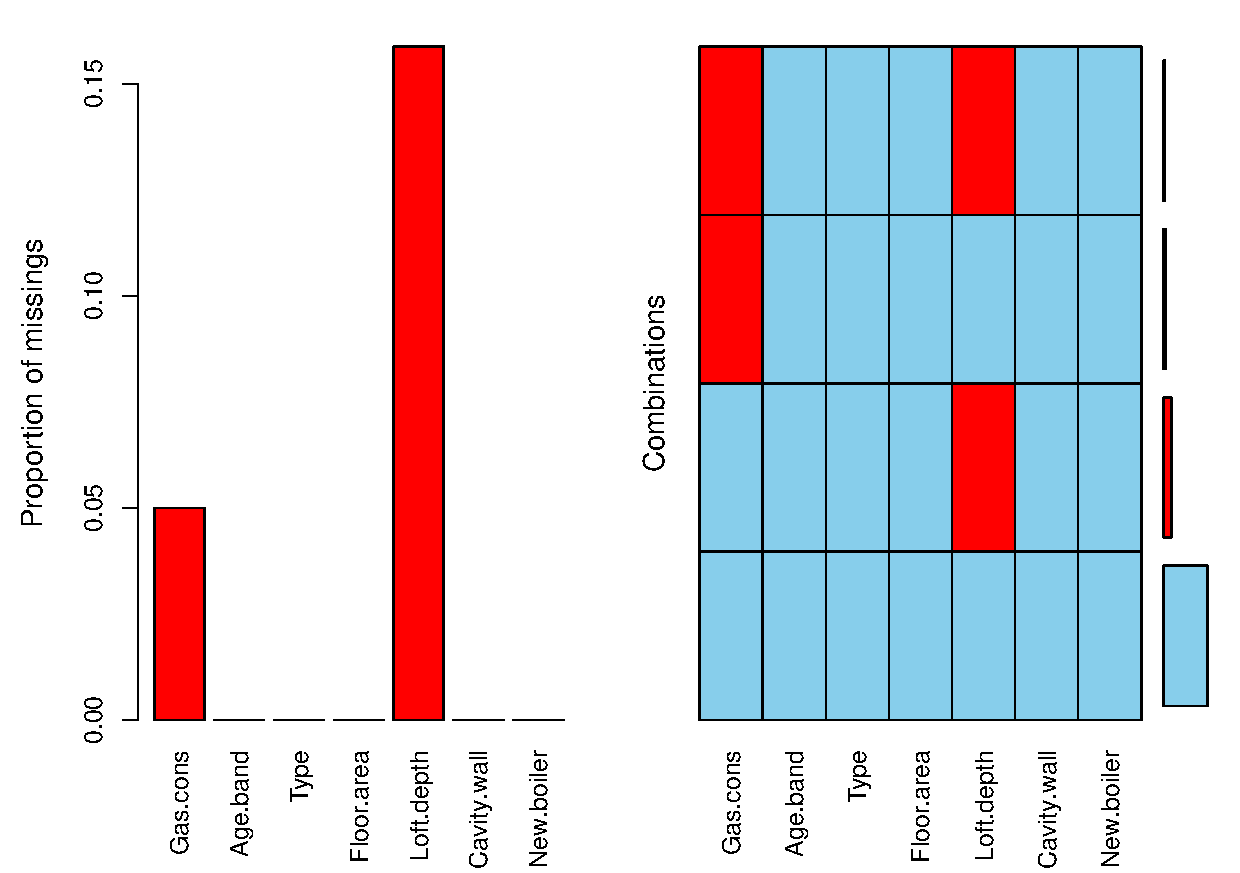
\includegraphics[width=0.7\textwidth]{aggre_missplot}
	\caption{Aggregate plot of missingness in our data}
	\label{fig:aggrmiss}
\end{figure}

\begin{figure}[H]
	\centering
	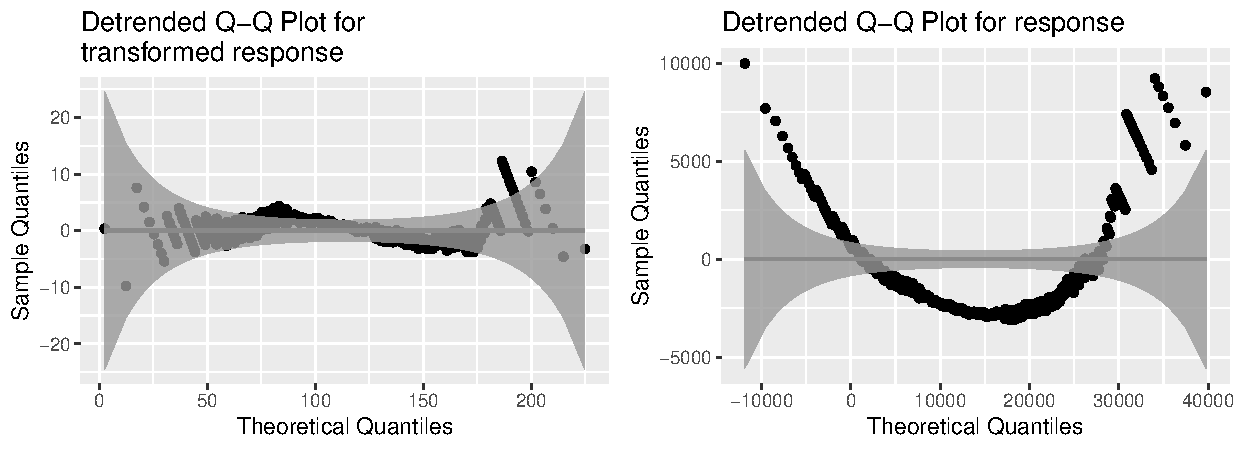
\includegraphics[width=0.7\textwidth]{qqplots}
	\caption{Model diagnostic plots for the transformed and non-transformed models}
	\label{fig:qqplots}
\end{figure}




\end{document}